%methods

\begin{figure*}[t]
\centering
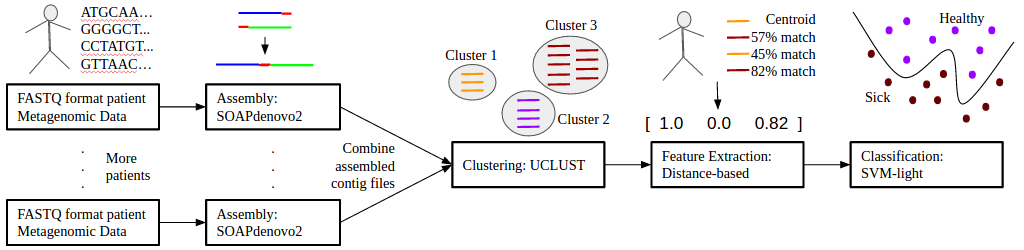
\includegraphics[scale=0.5]{./mil-metagenomics-pipeline.png}
\caption{This diagram illustrates the entire CAMIL pipeline. Patient files with FASTQ metagenomic reads are individually assembled using SOAPdenovo2, then combined into one file and clustered with UCLUST. We extract features according to either the D-BoW or H-BoW method, and classify the patients using the feature vectors with svm-light.} \label{pipeline}
\end{figure*}

\subsection{Overview}

Our proposed pipeline involves a number of steps, which serve a variety of purposes. For each patient file, we assembled the sequence reads, which served the dual purpose of generating larger contigs that contain more functional biological information and reducing the dataset size by discarding reads that could not be assembled. The clustering step assigns the contigs to certain clusters, which represent functionally similar microbes, and thus establish classes of instances that can be used as features for the classifier. We then developed a vocabulary-based feature extraction method.

Vocabulary-based methods are Bag of Words (BoW) methods, which involve the following three-step process: (i) Cluster the instances to create classes of instances; (ii) for each bag, map the clusters of instances in that bag to a feature vector; and (iii) use a standard classifier that uses the feature vectors to predict group labels \cite{amores13}. Amores found the Distance-based Bag of Words (D-BoW) method to be the second most effective of all tested methods, and the most effective one that was also time-efficient (linear, rather than quadratic, in the number of bags and number of instances per bag) \cite{amores13}. The distinguishing feature in D-BoW methods is that the values for the feature vector represent the instance that has the smallest distance to the cluster center. Histogram-based Bag of Words (H-BoW) methods count the number of instances from each cluster there are in each bag, instead of keeping track of the closest-matching instance to that cluster. This intuitively has appeal in the domain of microbiome analysis, as the relative quantities of different species of bacteria is important. H-BoW methods were found by Amores to be somewhat less effective than D-BoW methods on average, but performed the best out of all algorithms on several datasets, indicating that this method performs very well on some real world problems \cite{amores13}.

Our feature extraction method uses either the Histogram-based or Distance-based BoW methods. We used an SVM-based classifier to predict patient phenotype, and used several metrics to assess its accuracy. We used the SVM's decision boundary to infer information about which clusters of instances were most or least indicative of the phenotype, discussed further in the Results section. Aside from the patient labels, this process is entirely de novo, and does not consult any external databases. An illustration of the pipeline is shown in Figure \ref{pipeline} on page \pageref{pipeline}.

\subsection{Assembly with SOAPdenovo2}

For our assembly step, we used SOAPdenovo2, because it was the assembler used in the original MGWAS study \cite{qin041012} and because it has been shown to be one of the fastest assembly algorithms \cite{peng12}. SOAPdenovo2 first constructs a type of directed graph called a \emph{de Bruijn} graph that represents the overlaps between different sequences \cite{li10}. Reads are divided into strings of length K called \emph{k-mers}; these k-mers are the nodes of the graph \cite{zerbino08}. The choice of K is up to the user, and is important for having good assembly results. The k-mer nodes in the graph have an edge between them if a read contains those k-mers in order with an overlap of K-1 nucleotides, and the direction of the edge indicates in which order the k-mers appear \cite{zerbino08}. SOAPdenovo2 then cleans this graph by removing nodes/sequences with few or no connections with other sequences, eliminating ``tips" that represent likely sequencing machine errors, and removing redundant edges \cite{li10}. This step helps to reduce the overall size of the data by eliminating some reads that would not have been useful anyway. The contigs are then formed by combining reads according to the de Bruijn graph: each contig represents a directed path in the graph \cite{zerbino08}. 

We tested a number of different combinations of parameters, and found that the best results came when we cut reads off after 100 base pairs (reads were 180 base pairs long originally) and used a k-mer size of 51. The average insert size was set to 350, in accordance with the reported average insert size from the MGWAS study that we used data from \cite{qin041012}. The patient files needed to be assembled separately, in order to avoid assembling reads from different patients together. Conversely, all contigs need to be in one file for clustering, to avoid inconsistent cluster assignments between different patients. Thus, we combined the contigs from each assembled patient file into a single for clustering.

\subsection{Clustering with UCLUST}

We use UCLUST within our study, which is one of the most widely used and cited metagenome clustering methods and has been shown to be amongst the most effective in terms of speed and accuracy in benchmarking studies \cite{bonder090112, sun042711}. UCLUST seeks to ensure that, for some similarity T, the following conditions hold: (i) all cluster centroids have a similarity of less than T to each other; and (ii) all points in a cluster have a similarity of greater than T to the cluster centroid \cite{Edgar10}. Thus, each \emph{centroid} defines the center of a cluster, and the distance T defines the radius of the cluster, such that any point that has a similarity of greater than T to the centroid is within the radius and is thus part of the cluster. UCLUST is a heuristic algorithm that has several optimizations to improve speed, thus condition (i) above is not always guaranteed \cite{Edgar10}. UCLUST proceeds in a greedy, iterative manner. The first sequence in the input file becomes a new cluster centroid. For each new sequence in the file, it is compared with each of the existing cluster centroids in order. As soon as it is compared with a centroid that it has a similarity of greater than T with, it becomes part of that cluster. If the read is not similar enough with any of the existing cluster centroids, it becomes the centroid of a new cluster. The similarity measure T is defined as a string similarity between the two nucleotide sequences that counts the number of character placements that they have in common and then divides that number by the length of the reads, with terminal characters excluded \cite{Edgar10}. 

Since our contigs were not ordered, we used the usersort option, and we set the sequence match threshold to 40\%, which means that two reads needed to have 40\% of the same nucleotides to be in the same cluster. For instance, between two strings of length 100, at least 40 places in each of those strings would have to contain the same nucleotide (represented as A, T, G, or C). New contigs that did not match at least 40\% to any of the existing contigs would form the seed of a new cluster. This value of 40\% was found to be the best value based on our experiments with this dataset. Other values tried, including 50\%, 75\%, and 90\%, led to many clusters with very few reads per cluster.

\subsection{Feature Extraction and Classification}

We test both the Distance-based and Histogram-based feature extraction methods within the CAMIL pipeline. For each patient, we initialized a vector with length equal to the number of clusters. The value for each scalar in that patient's feature vector would then represent either the read that matched most closely to that cluster centroid (Distance-based), or the number of reads from that cluster that were present (Histogram-based. An example of this is illustrated as a part of Figure \ref{pipeline}. We implemented this feature extraction method in Python. We performed classification with a standard SVM classifier using the generated feature vectors; in this case, we used svm-light \cite{joachims08}. The choice of classifier is not very important for D-BoW methods \cite{amores13}.

\subsection{Deriving Instance ``Labels"}

\begin{figure}[t]
\centering
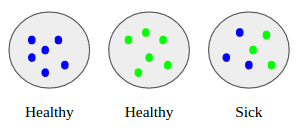
\includegraphics[scale=0.5]{./instance-labels.png}
\caption{This diagram illustrates why static instance labels are not sufficient for phenotype prediction. A patient with 6 of the blue microbe or 6 of the green microbe may be healthy, while a patient with 3 of each is sick. Static instance labels cannot capture this relationship. This is also explained by Amores in his MIL taxonomy \cite{amores13}.} \label{instance-labels}
\end{figure}

One of the benefits of using Multiple Instance Learning methods is that we can attempt to discover instance ``labels". In fact, we did not attempt to apply static, unchanging labels to individual reads or clusters, since organisms are affected by their interactions with each other. For instance, a patient with X amount of microbe A or X amount of microbe B may be healthy, but with X/2 amount of microbe A and X/2 amount of microbe B they may be sick. This simple example is illustrated in Figure \ref{instance-labels}. We can infer from the SVM decision boundary which clusters appear to be most relevant to the disease diagnosis. Since feature vectors are multiplied by the weight vector of the decision boundary to determine the label of the patient, we can assume that clusters with the highest weights in the weight vector are most relevant to the disease diagnosis. For instance, if the \emph{i}th scalar in the weight vector is has the highest value of any of the weights, then cluster \emph{i} is likely to play a major role in the disease pathology. Similarly, the most negative weights in the weight vector indicate clusters whose presence in a patient indicates that they likely do not have the disease. Because the data is metagenomic, the clusters represent both phylogenetic and functional similarity, so identifying the most relevant clusters can help discover more about the pathology of the disease. For Type 2 Diabetes, which is a complex phenotype and a disease that is both common and deadly, this is potentially quite valuable.